%!TEX root =  Write_a_classifier.tex

One of the main challenges for scaling up object recognition systems is the lack of annotated images for real-world categories. 
%It is estimated that humans can recognize and discriminate among about 30,000 categories~\cite{biederman1987recognition}. 
Typically there are few images available for training classifiers for most of these categories. This is reflected in the number of images per category available for training in most object categorization datasets, which, as pointed out in~\cite{Salakhutdinov11}, shows a Zipf distribution. 
The problem of lack of training images becomes even more severe when we target recognition problems within a general category, \ie, fine-grained categorization, for example building classifiers for different bird species or flower types  (there are estimated over 10000 living bird species, similar for flowers). 
Researchers try to exploit shared knowledge between categories to target such scalability issue.
This motivated many researchers who looked into approaches that learn visual classifiers from few examples, \eg~\cite{deng2010does,fe2003bayesian,BartU05}.   This even motivated a more recent work on zero-shot learning of visual categories where there are no training images available for test categories (unseen classes), \eg~\cite{Lampert09}. Such approaches exploit the similarity (visual or semantic) between seen classes and unseen ones, or describe unseen classes in terms of a learned vocabulary of semantic visual attributes. 


  \begin{figure}[t!]
\centering
\vspace{-3mm}
    \includegraphics[width=0.83\linewidth]{figproblem2.png} 
      \vspace{-2mm}
  \caption{{Our proposed setting where machine can predict unseen class from class-level unstructured  text description}}
  \label{fig:problem}
    \vspace{-6mm}
\end{figure}

In contrast to the lack of reasonable size training sets for a large number of real world categories, there are abundant of textual descriptions of these categories. This comes in the form of dictionary entries, encyclopedia articles, and various online resources. For example, it is possible to find several good descriptions of a ``bobolink'' in encyclopedias of birds, while there are only a few images available for that bird online. 

{\em The main question we address in this paper is how to use purely textual description of categories with no training images to learn visual classifiers for these categories.} In other words, we aim at zero-shot learning of object categories where the description of unseen categories comes in the form of typical text such as an encyclopedia entry; see figure~\ref{fig:problem}. We explicitly address the question of how to automatically decide which information to transfer between classes without the need of human intervention.  In contrast to most related work, we go beyond the simple use of tags and image captions, and apply standard Natural Language Processing techniques to typical text to learn visual classifiers. 


Fine-grained categorization \ignore{(also known as subordinate categorization)} refers to classification of highly similar objects. This similarity can be due to natural intrinsic characteristics of subordinates of one category of objects (e.g. different breeds of dogs) or artificial subcategories of an object class (different types of airplanes). Diverse applications of fine-grained categories range from classification of natural species~\cite{wah2011caltech,Flower08,wang2009learning,liu2012dog} to retrieval of different types of commercial products~\cite{maji2013fine}. 
\begin{figure*}[t]
\centering

%!TEX root =  NLPVision_proposal.tex

%\begin{figure}

\parbox{5.5in}{
\tiny
{\sf
The Bobolink (Dolichonyx oryzivorus) is a small New World blackbird and the only member of genus Dolichonyx.

\vspace{2pt}
Description: Adults are 16-18 cm (6-8 in) long with short finch-like bills. They weigh about 1 oz. Adult males are mostly black, although they do display creamy napes, and white scapulars, lower backs and rumps. Adult females are mostly light brown, although their coloring includes black streaks on the back and flanks, and dark stripes on the head; their wings and tails are darker. The collective name for a group of bobolinks is a chain.

\vspace{2pt}
Distribution and movement: These birds migrate to Argentina, Bolivia and Paraguay. One bird was tracked flying 12,000 mi over the course of the year, and up to 1,100 mi in one day. They often migrate in flocks, feeding on cultivated grains and rice, which leads to them being considered a pest by farmers in some areas. Although Bobolinks migrate long distances, they have rarely been sighted in Europe-like many vagrants from the Americas, the overwhelming majority of records are from the British Isles. 
Each fall, Bobolinks gather in large numbers in South American rice fields, where they are inclined to eat grain. This has earned them the name "ricebird" in these parts. However, they are called something entirely different in Jamaica (Butterbirds) where they are collected as food, being that they are very fat as they pass through on migration.


\vspace{2pt}
Behavior:
Their breeding habitats are open grassy fields, especially hay fields, across North America. In high-quality habitats, males are often polygynous. Females lay 5 to 6 eggs in a cup-shaped nest, which is always situated on the ground and is usually well-hidden in dense vegetation. Both parents feed the young. 
Bobolinks forage on or near the ground, and mainly eat seeds, insects, cultivated grains and rice.
Males sing bright, bubbly songs in flight; these songs gave this species its common name.
}}
\parbox{1.4in}{
\centering
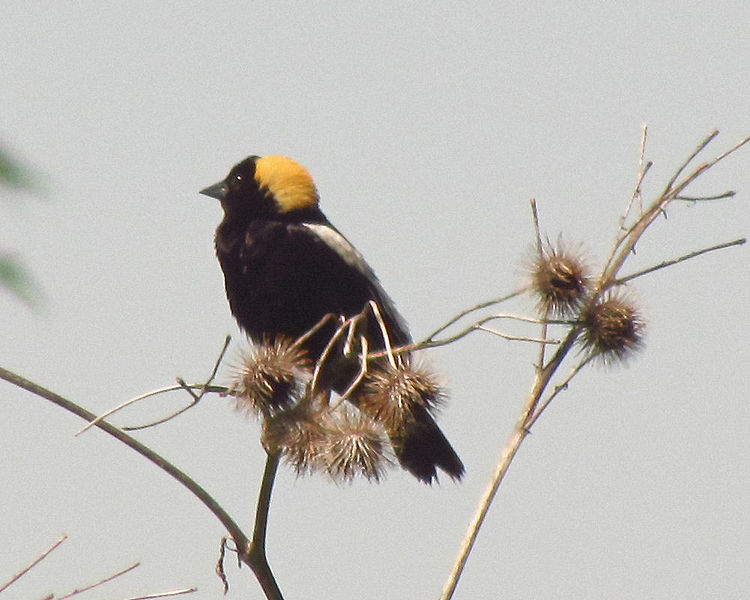
\includegraphics[width=1.2in]{Bobolink.jpg}
%\tiny {\sf (male)}
}
%\end{figure}

%\includegraphics[width=0.98\linewidth,height=.33\linewidth]{fig2_NLP.pdf}
\includegraphics[width=0.92\linewidth,height=.46\linewidth]{probDef_overall.png}
%\caption{Problem Definition: Zero-shot learning with textual description. Left: synopsis of textual descriptions for bird classes. Middle: images for ``seen classes''. Right: classifier hyperplanes in the feature space. The goal is to estimate a new classifier parameter given only a textual description}
\caption{ Top: Example Wikipedia article about the Painted Bunting, with an example image. Bottom: The proposed learning setting. For each category we are give one (or more) textual description (only a synopsis of a larger text is shown),  and a set of training images. Our goal is to be able to predict a classifier for a  category based only on the narrative (zero-shot learning). }
\label{F:prob_def}
\vspace{-14pt}
\end{figure*}
%Let us consider the problem of subordinate categorization of bird species as a case example. 
In this problem, When we learn from an expert about different species of birds, the teacher will not just give you sample images of each species and their class labels; the teacher will tell you about discriminative visual or non-visual features for each species, similarity and differences between species, hierarchal relations between species, and many other aspects. The same learning experience takes place when you read a book or a web page to learn about the different species of birds; For example, Fig.~\ref{F:prob_def} shows an example narrative about the {\sf Bobolink}. Typically, the narrative tells you about the bird's taxonomy, highlights discriminative features about that bird and discusses similarities and differences between species, as well as within-species variations (male vs. female). The narrative might eventually show very few example images, which are often selected wisely to illustrate certain visual aspects that might be hard to explain in the narrative.  This learning strategy using textual narrative and images makes the learning effective without a huge number of images  that a typical visual learning algorithm would need to learn the class boundaries. 
 
 





%Unnecessary details in images and text
 
%Although a narrative about a specific species can give very useful hints about what to look for to identify instances of that category, it also typically gives abundant of information about the species such as its habitat, diet, mating habits, etc. Such information is typically not useful for the task of the identification/recognition. In a sense, this information might be textual clutter for that task.  The same problem takes place in images, while one image can be very effective in highlighting an important feature for learning; typically images would have a lot of visual clutter that makes their uses in learning not effective. Many images of a given class might not provide discriminative features, and in fact can cause more confusion to a classifier. The point is a picture can worth a thousand words, but not always, and abundant of pictures might not be the most effective way for learning. Similarly one text paragraph can worth a thousand pictures for learning a concept, but not always, and abundant of text is not necessarily effective.  

%\begin{figure*}[t]
%
%!TEX root =  NLPVision_proposal.tex

%\begin{figure}

\parbox{5.5in}{
\tiny
{\sf
The Bobolink (Dolichonyx oryzivorus) is a small New World blackbird and the only member of genus Dolichonyx.

\vspace{2pt}
Description: Adults are 16-18 cm (6-8 in) long with short finch-like bills. They weigh about 1 oz. Adult males are mostly black, although they do display creamy napes, and white scapulars, lower backs and rumps. Adult females are mostly light brown, although their coloring includes black streaks on the back and flanks, and dark stripes on the head; their wings and tails are darker. The collective name for a group of bobolinks is a chain.

\vspace{2pt}
Distribution and movement: These birds migrate to Argentina, Bolivia and Paraguay. One bird was tracked flying 12,000 mi over the course of the year, and up to 1,100 mi in one day. They often migrate in flocks, feeding on cultivated grains and rice, which leads to them being considered a pest by farmers in some areas. Although Bobolinks migrate long distances, they have rarely been sighted in Europe-like many vagrants from the Americas, the overwhelming majority of records are from the British Isles. 
Each fall, Bobolinks gather in large numbers in South American rice fields, where they are inclined to eat grain. This has earned them the name "ricebird" in these parts. However, they are called something entirely different in Jamaica (Butterbirds) where they are collected as food, being that they are very fat as they pass through on migration.


\vspace{2pt}
Behavior:
Their breeding habitats are open grassy fields, especially hay fields, across North America. In high-quality habitats, males are often polygynous. Females lay 5 to 6 eggs in a cup-shaped nest, which is always situated on the ground and is usually well-hidden in dense vegetation. Both parents feed the young. 
Bobolinks forage on or near the ground, and mainly eat seeds, insects, cultivated grains and rice.
Males sing bright, bubbly songs in flight; these songs gave this species its common name.
}}
\parbox{1.4in}{
\centering
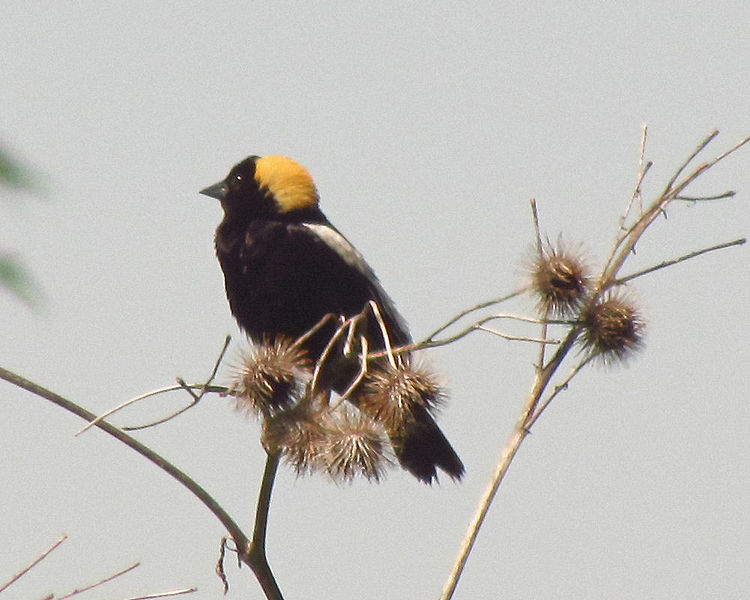
\includegraphics[width=1.2in]{Bobolink.jpg}
%\tiny {\sf (male)}
}
%\end{figure}


%\vspace{0.4cm}
%\includegraphics[width=0.99\linewidth,height=.27\linewidth]%{Text_vision_problemdef2.pdf}
%\label{F:prob_def}
%\vspace{-0.3cm}
%\caption{\footnotesize Top: Example Wikipedia article about the Painted Bunting, with an example image. Bottom: The proposed learning setting. For each category we are give one (or more) textual description (only a synopsis of  a larger text is shown),  and a set of training images. The first goal is to learn classifiers and detector for each bird species  jointly from the narrative and the images. A second goal  is to be able to predict a classifier and/or detector for a bird category only based only on the narrative (zero-shot learning). }
%\vspace{-15pt}
%\end{figure*}




%SM I changed slightly the above (I kept if need to get back to)
However, a narrative about a specific species does not contain only ``visually" relevant information, but also gives abundant information about the species's habitat, diet, mating habits that is not relevant for visual identification. In a sense, this information might be textual clutter for that task. The same problem takes place in images. While one image can be very effective in highlighting an important feature for learning, many images  might have a lot of visual clutter that makes their uses in learning not effective. %Many images of a given class might not provide discriminative features, and in fact can cause more confusion to a classifier. 
Thus, a picture can be worth a thousand words, but not always, and an abundant number of pictures might not be the most effective way for learning. Similarly, one text paragraph can be worth a thousand pictures for learning a concept, but not always, and large amounts of text might not necessarily be effective.





 

\textbf{Contributions.} The contribution of the paper is on exploring this new problem, which to the best of our knowledge, is firstly explored in the computer vision community in this work. We learn from an image corpus and a textual corpus, however not in the form of image-caption pairs, instead the only alignment between the corpora is at the level of the category. In particular, we address the problem of formulating a visual classifier prediction function ${\Phi (\cdot)}$, which predicts a  classifier of unseen visual class given its text description; see figure~\ref{F:prob_def}.  While a part of this work was  published in~\cite{Hoseini13}, we extend the work here to study more formulations to solve the problem in Sec.~\ref{formulation} (B,E). In addition, we also propose a kernel method to explicitly  predict a kernel classifier  in the form defined in the representer theorem~\cite{rth01}.  The kernelized prediction has an advantage that it opens the door for using any kind of side information about classes, as long as kernels can be used on the side information representation.  The side information can be in the form of textual, parse trees, grammar, visual representations, concepts in the ontologies (adopted in NLP domain), or any form. We focus here on unstructured text descriptions.\ignore{; see figure~\ref{fig:problem}} The image features also do not need to be in a vectorized format. The kernelized classifiers also facilitates combining different types of features through a multi-kernel learning (MKL) paradigm, where the fusion of different features can be effectively achieved.

\ignore{We propose and investigate two baseline formulations based on regression and domain adaptation. Then we propose a new constrained optimization formulation that combines a regression function and a knowledge transfer function with additional constraints to solve the problem.} 

Beyond the introduction and the related work sections, the paper is structured as follows: Sec~\ref{obvformulation} and ~\ref{sec_reganKT} details the problem definition and relation to regression and knowledge transfer models. Sec~\ref{formulation} shows different formulations of $\Phi(\cdot)$ that we studied to predict a linear visual classifier; see figure~\ref{F:prob_def}. Section~\ref{sec:app} developed extends our notion where  $\Phi(\cdot)$ predicts kernel classifier in the form defined by the representer theorem~\cite{rth01}. Sec~\ref{dskernel} presents our proposed distributional semantic kernel  between unstructured text description, which is applicable to  our kernel formulation and could be useful for other applications. Sec~\ref{experiments} presents our experiments  on Flower Dataset~\cite{Flower08} (102 classes) and Caltech-UCSD dataset~\cite{CU20010} (200 classes) for both the linear and the kernel classifier prediction.


